\documentclass[a4paper, 11pt]{book}

\usepackage[top=2cm,bottom=2cm,left=2cm,right=2cm]{geometry}
\usepackage[pdftex]{graphicx} %per poter inserire le figure
\usepackage{amssymb,amsmath,amsthm,amsfonts}
\usepackage[colorlinks=true, linkcolor=blue, citecolor=blue, urlcolor=blue]{hyperref}
\usepackage{xspace}
\usepackage{tabularx}
\usepackage{indentfirst}
\usepackage{subfigure}
\usepackage[small]{caption}
\usepackage{eucal}
\usepackage{eso-pic}
\usepackage{url}
\usepackage{booktabs}
\usepackage{afterpage}
\usepackage{parskip}
\usepackage{listings}
\usepackage{textcomp}
\usepackage{cite}
\usepackage{multirow}
\usepackage{subfiles} % Best loaded last in the preamble
\usepackage[utf8]{inputenc}   %per riuscire a scrivere gli accenti
\usepackage[italian]{babel}   %per riuscire a scrivere gli accenti
\usepackage{setspace} 
\usepackage{siunitx}
\usepackage{comment}
\usepackage{array}


\begin{document}
\begin{titlepage}
\vspace{5mm}
\begin{figure}[hbtp]
\centering

\includegraphics[scale=.13]{../Immagini/unipd_logo.png}
\end{figure}
\vspace{5mm}
\begin{center}
{{\huge{\textsc{\bf UNIVERSIT\`A DEGLI STUDI DI PADOVA}}}\\}
\vspace{5mm}
{\Large{\bf Dipartimento di Fisica e Astronomia ``Galileo Galilei''}} \\
\vspace{5mm}
{\Large{\textsc{\bf Corso di Laurea in Fisica}}}\\
\vspace{20mm}
{\Large{\textsc{\bf Tesi di Laurea}}}\\
\vspace{30mm}
\begin{spacing}{3}
{\LARGE \textbf{Proprietà dei candidati Muoni del Trigger L1 di CMS}}\\
\end{spacing}
\vspace{8mm}
\end{center}

\vspace{20mm}
\begin{spacing}{2}
\begin{tabular}{ l  c  c c c  cc c c c c  l }
{\Large{\bf Relatore}} &&&&&&&&&&& {\Large{\bf Laureando}}\\
{\Large{\bf Prof./Dr. Nome Cognome}} &&&&&&&&&&& {\Large{\bf Francesco La Rovere}}\\
{\Large{\bf Correlatore}}\\
{\Large{\bf Prof./Dr. Nome Cognome}}\\
\end{tabular}
\end{spacing}
\vspace{15 mm}

\begin{center}
{\Large{\bf Anno Accademico 2023/2024}}
\end{center}
\end{titlepage}
\clearpage{\pagestyle{empty}\cleardoublepage}

\frontmatter
\tableofcontents

\chapter*{Abstract}
\addcontentsline{toc}{chapter}{Abstract}
Dalla primavera del 2024 a CMS e' in produzione un sistema per acquisire a 40 MHz (ovvero senza filtro di trigger) i dati relativi ad i candidati oggetti fisici ricostruiti dal sistema di trigger di primo livello; tale sistema e' indicato come L1 Trigger Data Scouting, L1DS. In particolare il L1DS raccoglie le informazioni dai vari passaggi della catena logica dedicata alla identificazione e misura dei muoni, sono in particolare a disposizioni i "segmenti" individuati da ciascuna stazione dello spettrometro e le tracce ottenute a partire da questi. Lo studio che si propone in questa tesi verte sull'analisi di questi dati, con l'obbiettivo di caratterizzarne le proprietà. Appurato che le performance siano compatibili con quanto atteso (sulla base del confronto con i dati sintetici prodotti con simulazioni Monte Carlo), si utilizzeranno questi dati per cercare tracce con uno sviluppo temporale piu' lungo dello standard (in particolare sviluppandosi su piu' "bunch crossing") al fine di mettere le basi per la ricerca di particelle esotiche "lente" ovvero prodotte con beta non vicino ad 1.

\mainmatter
\chapter{Introduzione}
\label{cap:Introduzione}

In questo studio sono presentate le proprietà dei candidati muoni derivanti dal sistema di Trigger di primo livello del CMS, noto come L1T. Questo ha lo scopo di filtrare gli eventi derivanti dalle collisioni di protoni in modo da ridurre il volume di dati da analizzare, mantenendo solamente gli eventi interessanti. Come sarà discusso nel Capitolo \ref{cap:PrimoCapitolo} ciò introduce un bias, ovvero un pregiudizio sui dati, mascherando possibili informazioni che potrebbero portare alla scoperta di fisica Oltre il Modello Standard. A questo scopo viene introdotto il sistema di Data Scouting nel L1T, ovvero un sistema che consente di raccogliere eventi derivanti dalle collisioni, seppur con una minore risoluzione, eseguendo una analisi a livello del L1T e lavorando parallelamente ad esso. Studiare questi eventi piuttosto che quelli in uscita dal Trigger comporta ovviamente una maggiore presenza di segnali di fondo, ma ciò viene eseguito senza introdurre nessun bias nei dati analizzati per la analisi. Il sistema di Data Scouting nel L1T verrà implementato definitivamente a CMS con l'upgrade di LHC, Phase 2, permettendo quindi un grosso passo in avanti verso la scoperta di Nuova Fisica. In previsione della Phase 2, durante la Run 3 a CMS è stato introdotto un sistema di Data Scouting apposito a livello del L1T che consente la validazione e la sperimentazione di nuovi algoritmi da implementare con l'upgrade di CMS.


Nel Capitolo \ref{cap:PrimoCapitolo} verrà quindi introdotto il Large Hadron Collider e il suo principale esperimento, il Compact Muon Solenoid locato a Cessy, in Francia nel punto di interazione 5. Particolare attenzione verrà posta sulle camere muoniche, che permettono la rilevazione di muoni a CMS, e sul sistema di Trigger. Verrà inoltre più dettagliatamente discusso il sistema di Data Scouting di CMS nella Sezione \ref{sec:DataScouting}. Particolare attenzione avrà anche la sezione sulla ricerca di Nuova Fisica \ref{sec:NewPhysics}.

Nel Capitolo \ref{cap:SecondoCapitolo} verranno presentati e validati i risultati del sistema di Data Scouting introdotto con la Run 3, studiando le informazioni rilevate dalle schede di acquisizione nei principali step di acquisizione, verificandone la conformità. Verrà inoltre eseguito uno studio approfondito sul confronto tra candidati muoni del sistema di tracking BMTF e i muoni del GMT, esaminando quindi le differenze. Alla fine del Capitolo \ref{cap:SecondoCapitolo} verrà presentato un breve confronto con i dati raccolti dal sistema di Data Scouting nell'anno 2023 \cite{CERNsummerSchool}, evidenziandone le principali differenze.

Nel Capitolo \ref{cap:TerzoCapitolo} verrà invece introdotto l'algoritmo utilizzato per la ricerca di eventi compatibili con i modelli alla base delle Heavy Stable Charged Particles, mostrando anche i principali risultati ottenuti.

Infine nel Capitolo \ref{cap:Conclusioni} verranno presentate le conclusioni ottenute dai risultati del presente studio. 




\chapter{Il progetto LHC:}


\section{Large Hadron Collider}
Formato da un anello di circonferenza pari a 27 km, il Large Hadron Collider (LHC), situato al CERN a Ginevra, Svizzera, è il più grande acceleratore di particelle mai costruito, disegnato con lo scopo di studiare collisioni tra protoni con un energia nel centro di massa $\sqrt{s} = 13.6$ TeV e una luminosità istantanea nominale $\mathcal{L} = 2 \times 10^{34}$ \si{cm^{-2} s^{-1}}, corrispondente ad un rate di interazioni tra protoni di 40MHz, ovvero una collisione ogni 25ns. L'intervallo temporale tra le collisioni è chiamato \textit{bunch crossing}, BX, ed è una unità di misura standardizzata: 1 BX = 25ns.


\begin{figure}[t]
  \centering
  \begin{minipage}[b]{0.45\textwidth}
      \centering
      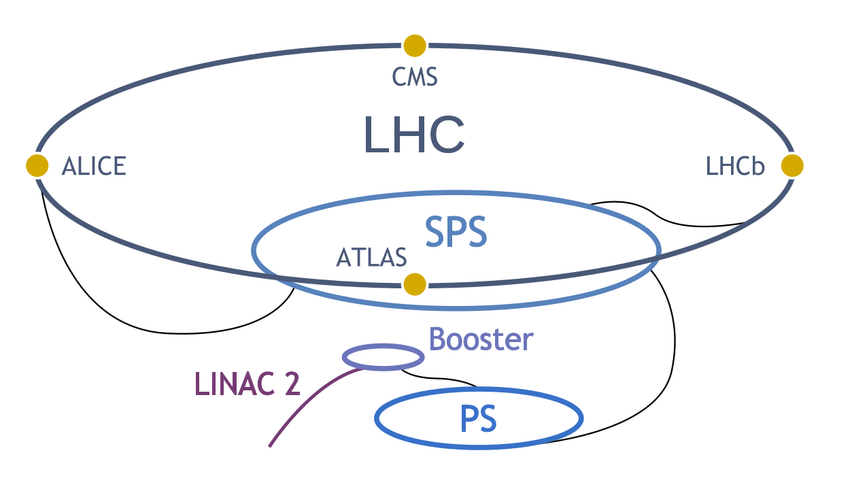
\includegraphics[width=\textwidth]{../ImmaginiTesi/LHC.png} 
  \end{minipage}
  \hfill 
  \begin{minipage}[b]{0.5\textwidth}
      \centering
      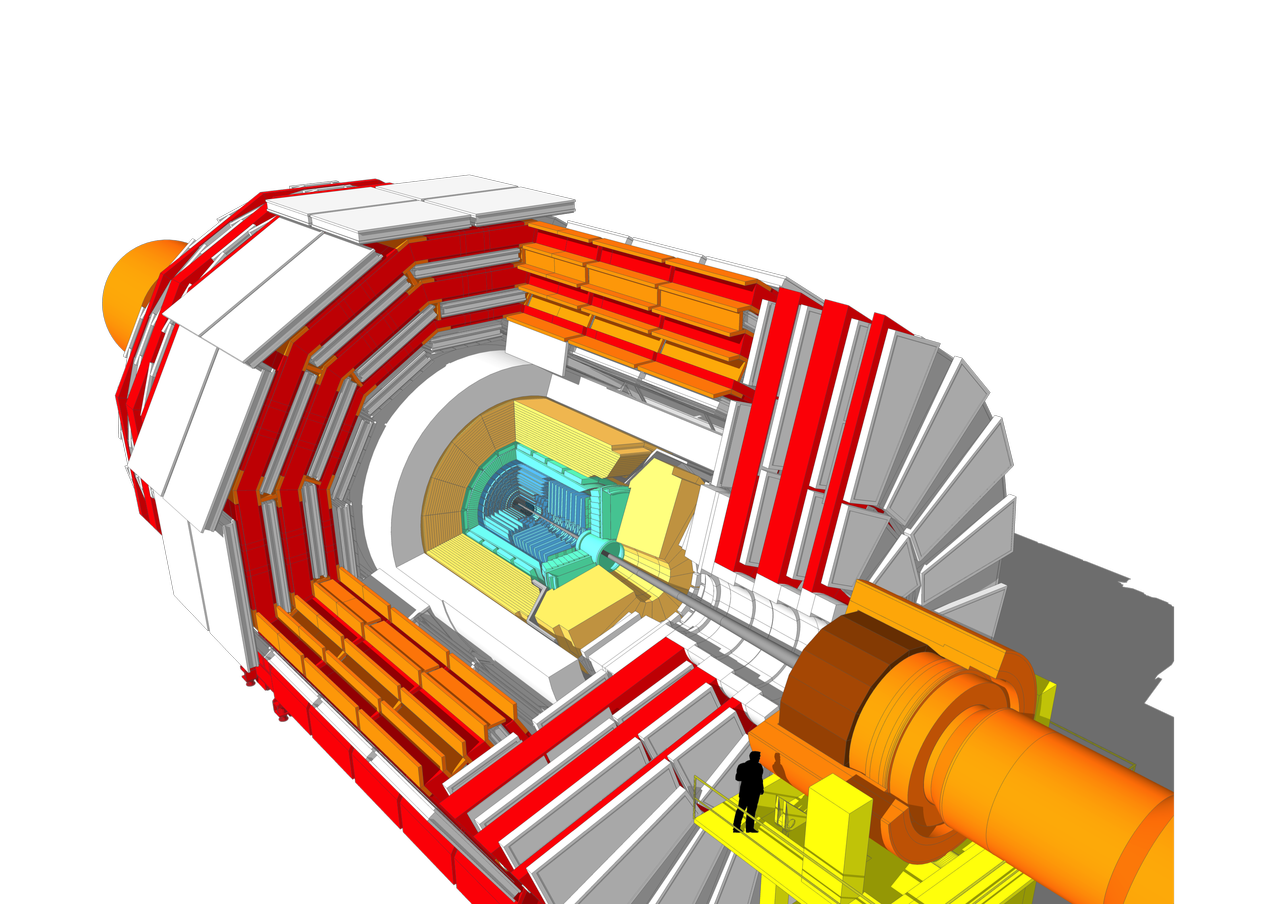
\includegraphics[width=\textwidth]{../ImmaginiTesi/CMS.png} 
  \end{minipage}
  \caption{Struttura dell'LHC e dei suoi rivelatori nei punti di interazione (sinistra), CMS (destra)}
  \label{fig:LHC-CMS}
\end{figure}


Prima di essere immessi in LHC, pacchetti formati da $1.1 \times 10^{11}$ protoni, subiscono varie fasi di accelerazione: inizialmente ad opera dell' acceleratore lineare Linac, poi dal Proton Synchrotron Booster (PSB), quindi dal Proton Synchrotron (PS) e infine dal Super Proton Synchrotron (SPS), dove vengono iniettati in LHC con una energia di 450 GeV. Circolando in due condotti differenti in direzioni opposte, i protoni vengono accelerati fino a 7 TeV collidendo frontalmente in punti di interazione con una energia nel centro di massa $\sqrt{s} \approx 14$ TeV. Come mostrato in Figura \ref{fig:LHC-CMS}, i principali punti di interazione dell'LHC sono: ATLAS (IP1), Alice (IP2), CMS (IP5) e LHCb (IP8).


L'LHC alterna periodi di fasi di attività e di raccolta dati (Run) con fasi di arresto in cui vengono effettuate opere di upgrade e di manutenzione. Tra la Run 1, iniziata nel 2009 e finita nel 2013, e la Run 2, tra 2015 e 2018, il sistema di trigger Level-1 (L1T) del CMS ha subito importanti miglioramenti (\textit{Phase 1}) rimpiazzando e potenziando hardware, elettronica e software del trigger permettendo, durante la Run 2, un incremento dell'energia di collisione protone protone nel centro di massa da 8 a 14 TeV \cite{sirunyan2020performance}. E' in programma nel 2025 un ulteriore upgrade dell'LHC (\textit{Phase 2}) che porterà un incremento della luminosità istantanea fino a $5\times 10^{34}$ \si{cm^{-2} s^{-1}}, aumentando quindi il numero di collisioni medio per BX da 50 a 140 \cite{collaboration2021phase}. In contemporanea, al fine di sfruttare appieno l'incremento della luminosità dell'LHC della Phase 2 (noto come \textit{HL-LHC}, High Luminosity LHC), è previsto un upgrade anche del sistema di detector del CMS, ed in particolare sul sistema di trigger L1, di cui parleremo nelle prossime sezioni.

\section{Compact Muon Solenoid}

%Il rivelatore CMS è formato da un corpo cilindrico di 15 m di diametro e 21.6 m di lunghezza, per un peso di circa 14.000 tonnellate ed è locato nel punto di interazione IP5 in Cessy, Francia.

Locato nel punto di interazione IP5 in Cessy, Francia, il CMS è formato da un corpo cilindrico di 15 m di diametro e 21.6 m di lunghezza, per un peso di circa 14.000 tonnellate \cite{cms2008cms}. Sono vari gli ambiti di ricerca del rilevatore nel campo della fisica delle alte energie: dopo la scoperta del bosone di Higgs nel 2012, misurare le sue proprietà, attualmente compatibili con il modello standard, è diventato di fondamentale importanza. Ugualmente rilevante è anche la ricerca e lo studio di particelle esotiche e supersimmetriche al fine di esplorare Nuova Fisica oltre il modello standard. (introduzione alle HSCP??)Al fine di identificare questi eventi è necessario un sistema di trigger molto performante \cite{sirunyan2020performance} e a questo scopo in gioco il nuovo sistema di trigger che verrà implementato nella \textit{Phase 2}, che permetterà quindi di osservare fenomeni esotici con una risoluzione migliore (assieme ad un nuovo sistema di analisi dati, \textit{Data Scounting}, di cui discuteremo maggiormente dopo aver introdotto il sistema di trigger del CMS (??))

Di seguito una panoramica della struttura del CMS, dalle componenti più interne fino a quelle più esterne \cite{MasterThesisNicLai}(Figura \ref{fig:LHC-CMS}):

\begin{itemize}
  \item \textbf{Silicon Strip Tracker (SST):} Esegue una ricostruzione delle tracce e misurazione del momento trasverso di particelle originate da processi di interazione. 
  \item \textbf{Electromagnetic Calorimeter (ECAL):} Misure di energia di fotoni ed elettroni vengono eseguite grazie al tungstato di piombo (\si{PbWO_4}), materiale scintillante di cui è costituito l'ECAL.
  \item \textbf{Hadronic Calorimeter (HCAL):} Permette la misurazione delle energie degli adroni grazie al fenomeno della \textit{cascata adronica}, indotta dai materiali di cui è costituito l'HCAL e rivelata da materiali scintillatori plastici.
  \item \textbf{Solenoide superconduttore:} Formato dal superconduttore Niobio-Titanio (NbTi), produce un campo magnetico di intensità 3.8T nel nucleo. Un campo magnetico così elevato è fondamentale per permettere la curvatura di particelle cariche prodotte dalle collisioni, la cui rivelazione di tale curvatura permette di risalire a momento e carica delle stesse.
  \item \textbf{Camere muoniche:} Suddiviso in tre regioni, \textit{barrel}, \textit{overlap} ed \textit{endcap}, il sistema delle camere muoniche copre il piano della pseudorapidità nel range $|\eta| < 2.4$, permettendo la rivelazione delle tracce di muoni usando tre diverse tecnologie: \textit{drift tubes} (DT), \textit{resistive plate chamber} (RPC) e \textit{cathode strip chamber} (CSC) \cite{TheMuonProject} (Figura \ref{fig:SectorEtaView}).
\end{itemize}


\subsection{Camere muoniche:}

\begin{figure}[t]
  \centering
  \begin{minipage}[b]{0.48\textwidth}
      \centering
      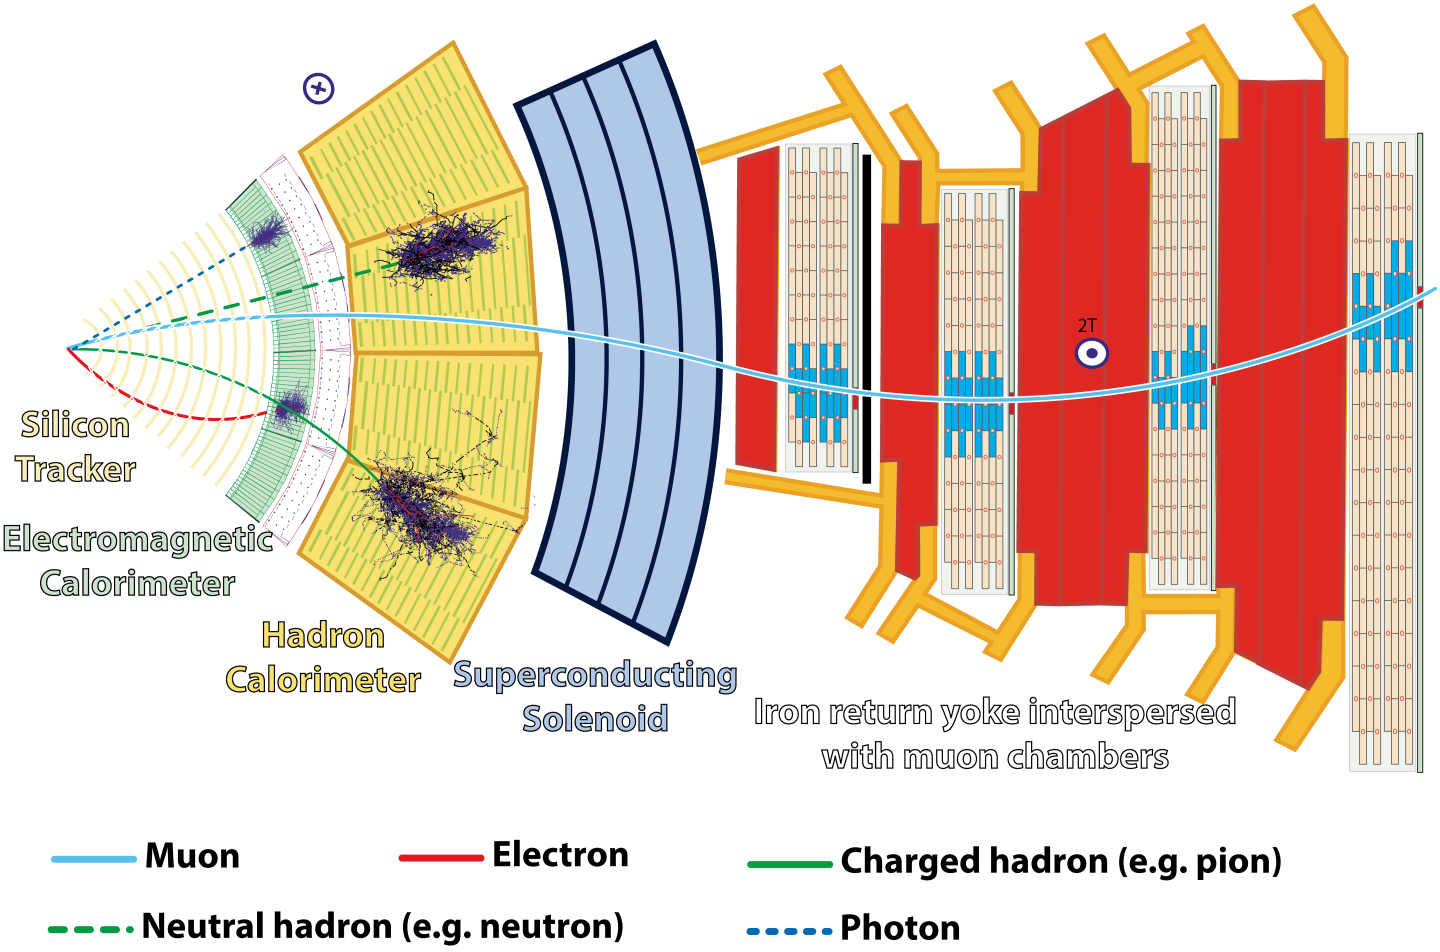
\includegraphics[width=\textwidth]{../ImmaginiTesi/CMS slice.png} 
  \end{minipage}
  \hfill 
  \begin{minipage}[b]{0.48\textwidth}
      \centering
      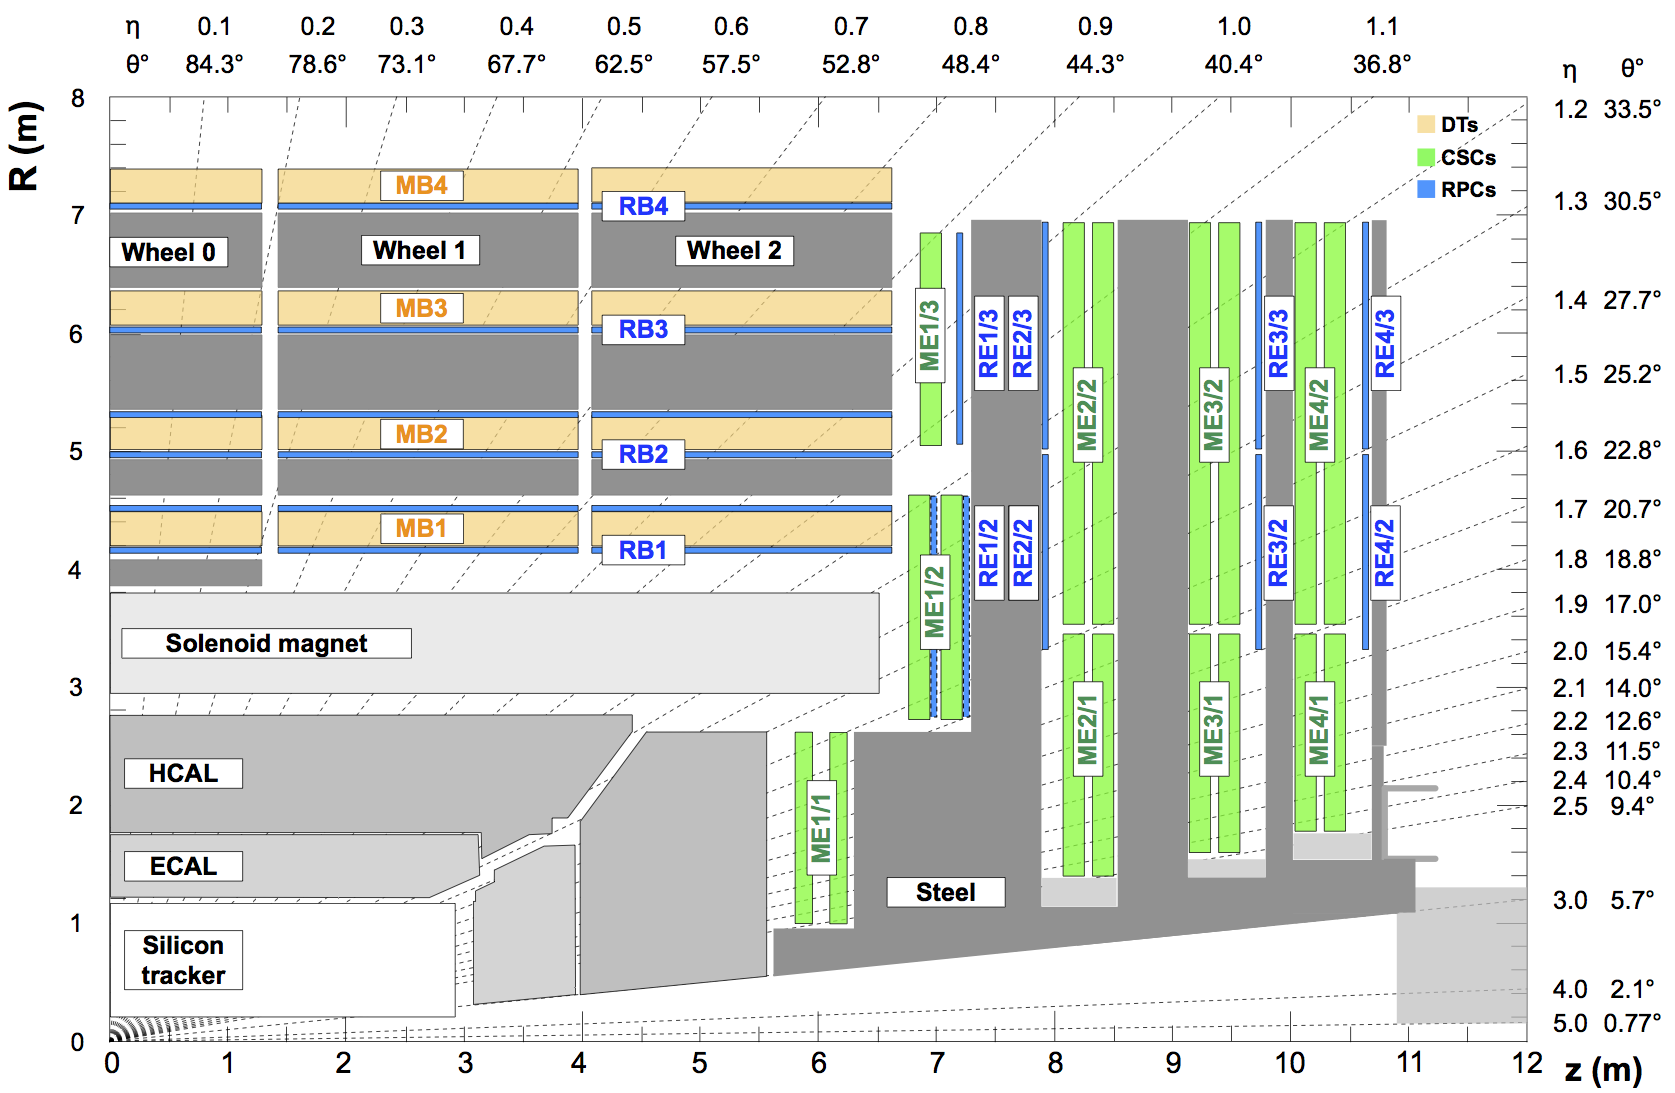
\includegraphics[width=\textwidth]{../ImmaginiTesi/CMSEtaView.png} 
  \end{minipage}
  \caption{Settore di CMS (sinistra), vista di CMS  nella variabile $\eta$ di CMS (destra)}
  \label{fig:SectorEtaView}
\end{figure}

L'alto rate di eventi di background a seguito di processi di interazione ad alta luminosità in LHC cela fenomeni interessanti: in questo contesto la rivelazione di muoni è uno strumento utile per studiare tali fenomeni. Una misurazione precisa di muoni è quindi di centrale importanza a CMS \cite{cms2008cms}. Il sistema muonico di CMS ha quindi tre funzioni: identificazione di muoni, misurazione del momento e trigger di muoni.

Il forte campo magnetico nella regione delle camere muoniche (figura \ref{fig:SectorEtaView}), permette una buona risoluzione del momento e capacità di trigger. (andrebbe aggiunto qualcosa)


In particolare la regione di barrel, come mostrato in figura \ref{fig:LHC-CMS} è formata da cinque ruote (\textit{wheel}), ognuna composta da dodici settori (\textit{sector}) e a loro volta ognuna da quattro stazioni concentriche (\textit{station}) interspaziate da una struttura di ferro. Nella regione di barrel, dove gli eventi di background sono minimi, per la rivelazione di muoni vengono impiegati drift tubes (DT), ricoprendo la pseudorapidità nel range $|\eta| < 1.2$. I DTs sono celle contenenti fili di acciaio inossidabile anodico disposte in modo adiacente una all'altra, separate da barre di alluminio che fungono da catodo: anodo e catodo operano ad un voltaggio rispettivamente di +3600V e -1200V. Quando un muone attraversa un DT la distanza di esso dal filo di acciaio viene misurata a partire dal tempo di drift degli elettroni ionizzati \cite{MasterThesisNicLai}. 
In totale il CMS contiene 250 DTs, disposti nella regione di barrel come in figura \ref{fig:SectorEtaView}. Nelle regioni di endcap di CMS, dove il rate di muoni e livello di background è elevato ed il campo magnetico non uniforme, vengono impiegate CSCs che, grazie al loro design, permettono di ricavare precise informazioni spaziali e temporali sulle tracce di muoni nel range di pseudorapidità $0.9 < |\eta| < 2.4$. Le RPCs sono invece impiegate sia nella regione di barrel che nella regione di endcap, e assicurano una migliore misurazione del momento dei muoni grazie al loro rapido tempo di risposta \cite{MasterThesisNicLai}, \cite{cms2008cms}.


\subsection{Sistema di trigger:}

Non è possibile analizzare in tempo reale la mole di informazioni generata dal tasso di collisioni pari a 40MHz, per questo CMS è dotato di un sistema di trigger implementato come primo passo nella selezione di un processo fisico. 

Al fine di ridurre il volume di dati, mantenendo però gli eventi interessanti, il sistema di trigger si suddivide in due fasi: il \textit{Level 1 Trigger} (L1T) e l' \textit{High Level Trigger} (HLT) (figura \ref{fig:TriggerSystem}). 

Il Level 1 Trigger è implementato via hardware nel sistema di CMS e, unendo informazioni del sistema muonico e del calorimetro, riduce il tasso di accetazione di eventi a 100KHz, mantenendo gli eventi che, in base a logiche interne, hanno qualità elevata. Il processo di selezione deve avvenire rapidamente, in un tempo limite di 25 ns, per permettere a tutti gli eventi di essere analizzati dal trigger e ridurre quindi il numero di possibili eventi mancati; per questo il sistema di trigger L1 è composto da tre processi: \textit{locale}, \textit{regionale} e \textit{globale} \cite{MasterThesisNicLai}.
Il sistema di trigger quindi raccoglie le informazioni \textit{locali} riguardanti i calorimetri elettromagnetici e adronici (ECAL, HCAL) e le informazioni sul sistema muonico (DTs, RPCs, CSCs). Le informazioni provenienti da processi locali sono chiamate Trigger Primitive Generators (TPG). Queste vengono combinate dai \textit{trigger regionali} che effettuano una classifica degli eventi sulla base di parametri come energia, momento e qualità. Quindi il \textit{trigger globale} (GT) determinerà se mantenere l'evento o se passarlo all' HLT.





\begin{figure}[t]
  \centering
  \begin{minipage}[b]{0.40\textwidth}
      \centering
      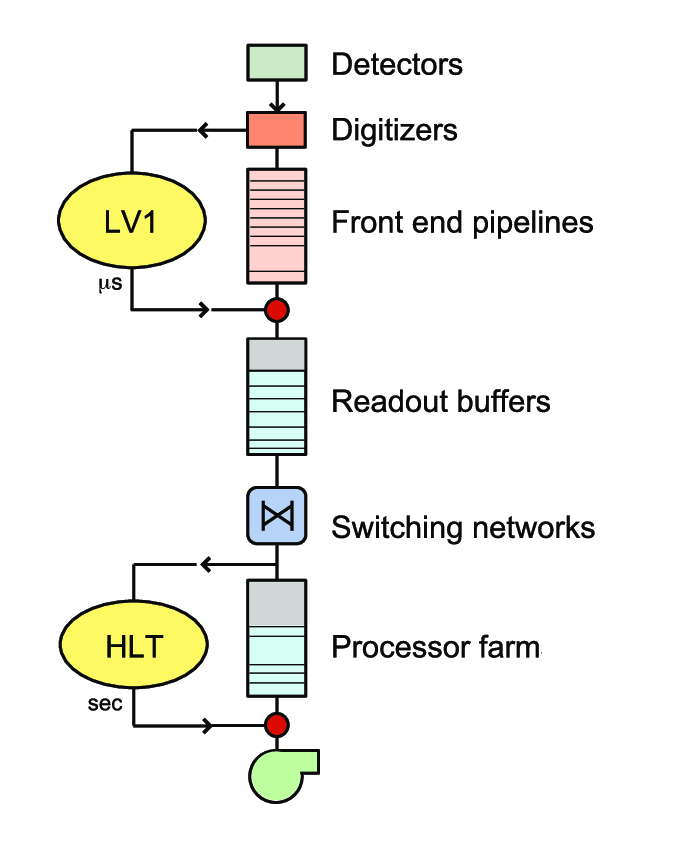
\includegraphics[width=\textwidth]{../ImmaginiTesi/TriggerSystem2.png} 
    \end{minipage}
    \hfill 
    \begin{minipage}[b]{0.48\textwidth}
      \centering
      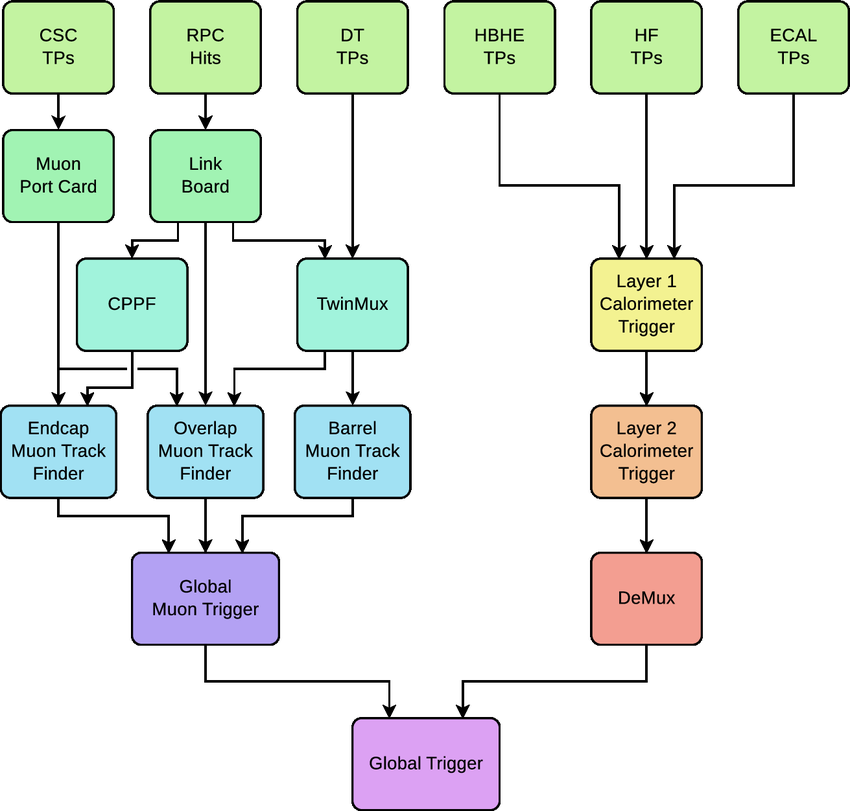
\includegraphics[width=\textwidth]{../ImmaginiTesi/TriggerSystem.png} 
  \end{minipage}
  \caption{}
  \label{fig:TriggerSystem}
\end{figure}















\appendix

\bibliographystyle{plain}
\bibliography{Bib}




\end{document}






